\chapter{Automated Manual Build}
\ChapterLabel{AutomatedBuild}
\index{Gitea Actions}
\index{automated manual build}

\section{Overview and Status}
This chapter answers the course manual's Chapter~3 \cite{DosManual}: every push
of this manual's LaTeX source to the team's Gitea repository builds the PDF on a
self-managed Gitea runner and publishes it as a downloadable artifact whose title
page and footers carry the commit and run that produced it. The eight numbered
subsections match the eight rubric rows in order.

\begin{tabularx}{\linewidth}{L{5.6cm}L{1.4cm}L{1.6cm}Y}
\caption{Rubric rows, owners, and status\label{Table:BuildStatus}}\\
\toprule \textbf{Subsection} & \textbf{Points} & \textbf{Owner} & \textbf{Status}\\ \midrule
\endfirsthead
\toprule \textbf{Subsection} & \textbf{Points} & \textbf{Owner} & \textbf{Status}\\ \midrule
\endhead \bottomrule \endlastfoot
Source and trigger & 15 & BD & \StatusPending\\
Runner setup & 15 & BD & \StatusPending\\
Reproducible compilation & 20 & SD & \StatusPending\\
PDF version traceability & 15 & SD & \StatusPending\\
Downloadable artifact & 10 & BD & \StatusPending\\
Change, failure, and repair evidence & 10 & SD & \StatusPending\\
Runner and secret boundary & 5 & BD & \StatusPending\\
Manual quality and controls & 10 & SD & \StatusPending\\
\end{tabularx}

\section{Required Subsections}
% ======================================================================
% Region: buildSourceTrigger (single owner; edit only your own region)
\subsection{Source and trigger (15 points)}
\label{Section:buildSourceTrigger}
\textbf{Owner:} BD. \StatusPending{}
\Todo{repository, main file and workflow links; branch and push event; HTTPS remote, port 443, Caddy, private port 3000; why the runner needs no public port; a run started by a push.}

% ======================================================================
% Region: buildRunner (single owner; edit only your own region)
\subsection{Runner setup (15 points)}
\label{Section:buildRunner}
\textbf{Owner:} BD. \StatusPending{}
\Todo{runner version, location, scope, label \texttt{manual-builder}, execution mode, network path, capacity; runner online and a job assigned; isolation; no public ports.}

% ======================================================================
% Region: buildCompilation (single owner; edit only your own region)
\subsection{Reproducible compilation (20 points)}
\label{Section:buildCompilation}
\index{TeX Live}
\index{latexmk}
\textbf{Owner:} SD. \textbf{Status:} successful build on the Gitea runner,
run~\#2, October 20, 2026, 03:00~UTC \StatusPass.

\subsubsection{Toolchain}
\begin{tabularx}{\linewidth}{L{4.0cm}Y}
\caption{Build toolchain\label{Table:BuildToolchain}}\\
\toprule \textbf{Item} & \textbf{Value}\\ \midrule
\endfirsthead
\toprule \textbf{Item} & \textbf{Value}\\ \midrule
\endhead \bottomrule \endlastfoot
Job image & \texttt{group1/texlive-node:2026.09}, built from \texttt{ci/Dockerfile}\\
Base image & \texttt{texlive/texlive}, pinned by digest \texttt{sha256:7334b00bf8e7\ldots 3083ff} (image created September 20, 2026)\\
TeX & TeX Live 2026, pdfTeX 3.141592653-2.6-1.40.29, \texttt{latexmk} 4.88\\
Other tools in the image & Python 3 with Pygments (\texttt{minted}), \texttt{bibtex}, \texttt{makeglossaries}, \texttt{makeindex}, \texttt{git}\\
Added for Actions & Node.js 24 (Debian package), needed by \texttt{actions/checkout} and \texttt{actions/upload-artifact}\\
Main file & \texttt{devopsITManual.tex} at the repository root\\
Build command & \texttt{latexmk -pdf -shell-escape -interaction=nonstopmode -halt-on-error -usepretex=\ldots{} devopsITManual.tex}\\
Expected output & \texttt{devopsITManual.pdf}, copied to \texttt{out/IT-manual+build.<run>.<sha>.pdf}\\
\end{tabularx}
TeX is installed only in the job image, which is stored in the server's
Docker engine; it is not in the Gitea container and not in the server's own
operating system. The runner starts a fresh container from that image for
each job and removes it afterwards.

\subsubsection{Workflow}
\inputminted{yaml}{.gitea/workflows/build.yml}

\subsubsection{Failure detection}
The build fails, and no artifact is uploaded, when:
\begin{itemize}[nosep]
  \item \texttt{pdflatex} reports any error: \texttt{-halt-on-error} stops it and \texttt{latexmk} exits non-zero;
  \item \texttt{devopsITManual.pdf} is missing or empty;
  \item the final pass still reports undefined or multiply defined references;
  \item the build identifier is not in the LaTeX log (row~4);
  \item no PDF matches the upload path (\texttt{if-no-files-found: error}).
\end{itemize}
Before pushing, the same commands were run in the same image on SD's
workstation (\texttt{ci/local-build.sh}): a clean build took about 18~seconds,
and a copy with an undefined command inserted exited with code~1, reported
``Undefined control sequence'' with the line number, and produced no PDF.

\subsubsection{Checkout and artifact path}
The runner polls Gitea over HTTPS for work. In the job container,
\texttt{actions/checkout} fetches the triggering commit from
\texttt{https://git.ssw590-g1.tech}, and \texttt{actions/upload-artifact} sends
the PDF back to the same run over HTTPS. Gitea and the job share no
filesystem.

\subsubsection{Runs on the server}
The first push (commit \texttt{1fb4e15},
\href{https://git.ssw590-g1.tech/group1-startup/manual/actions/runs/1}{run~\#1})
compiled the manual but failed at the upload step: Gitea~1.27.3 rejects
\texttt{actions/upload-artifact@v4} with ``GHESNotSupportedError''. Version~3 of
the action is supported, so commit \texttt{a5f3446} changed only that line, and
\href{https://git.ssw590-g1.tech/group1-startup/manual/actions/runs/2}{run~\#2}
succeeded (\FigRef{61}, \ListRef{62}). The compile step took 36~seconds on the
\texttt{t3.micro} server, and the whole job 1~minute 11~seconds, including
24~seconds to start the job container. The run pages and the full job logs are
public, so they can be opened without an account.

\begin{figure}[htbp]
\centering
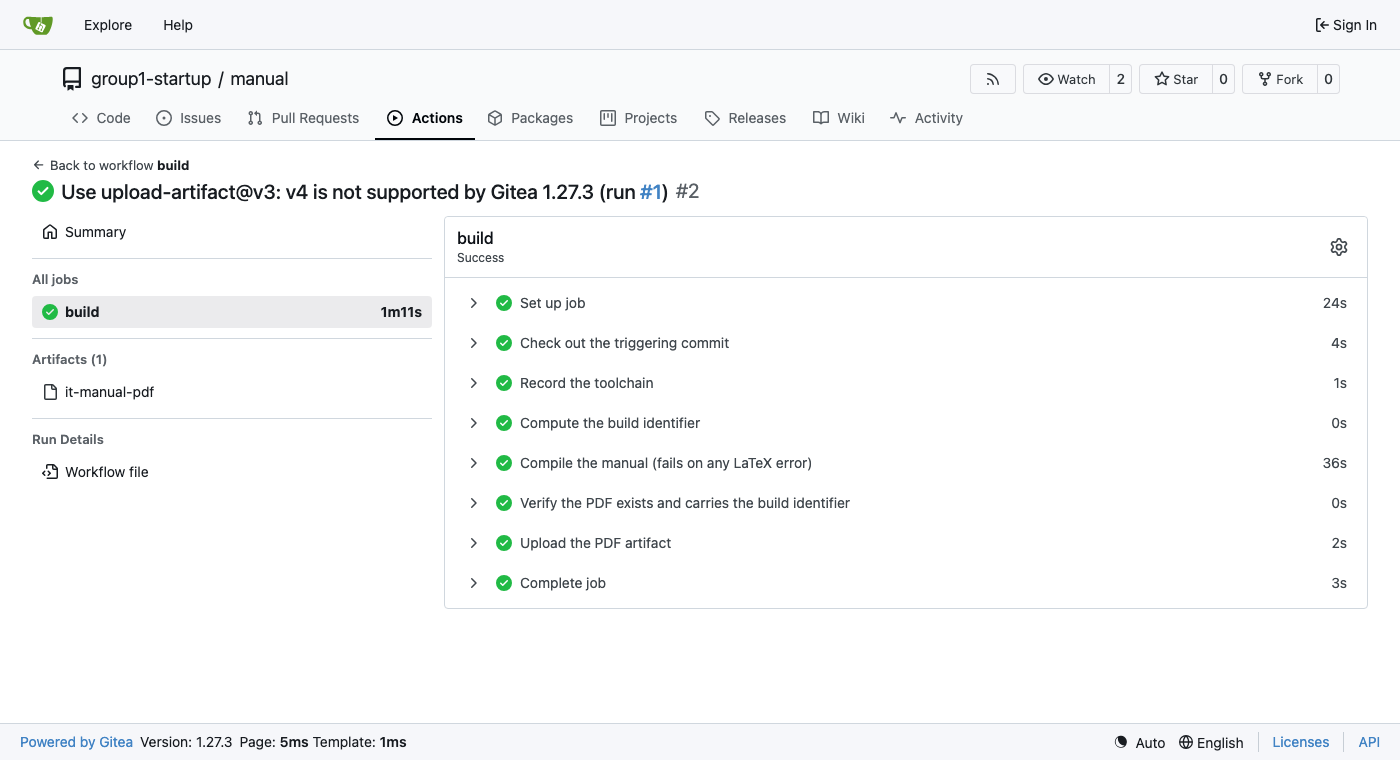
\includegraphics[width=0.9\linewidth]{evidence/61-run2-job-steps-success-a5f3446-2026-10-20.png}
\caption{\href{https://git.ssw590-g1.tech/group1-startup/manual/actions/runs/2}{Run~\#2} on the Gitea runner, October 20, 2026, seen signed out: every step succeeded and the run has one artifact, \texttt{it-manual-pdf}.}
\label{Fig:E61}
\end{figure}

\begin{longlisting}
\inputminted[fontsize=\scriptsize]{text}{evidence/62-run2-log-excerpt-success-a5f3446-2026-10-20.txt}
\caption{Run~\#2: step results from the Gitea API and key lines of the job log (toolchain versions, build identifier, compile passes, artifact upload), October 20, 2026.}
\label{Listing:E62}
\end{longlisting}

% ======================================================================
% Region: buildTraceability (single owner; edit only your own region)
\subsection{PDF version traceability (15 points)}
\label{Section:buildTraceability}
\textbf{Owner:} SD. \textbf{Status:} identifier verified on the PDF
downloaded from run~\#2 \StatusPass.

The human-maintained version stays \texttt{\string\DocumentVersion} in
\texttt{devopsITManual.tex}, changed only by a person with a history entry. The
workflow appends a build suffix
\texttt{+build.<run\_number>.<first 7 characters of the commit>}, taken from
Gitea's \texttt{gitea.run\_number} and \texttt{gitea.sha} \cite{GiteaActionsVars}.
It reaches LaTeX through \texttt{latexmk -usepretex}, which defines
\texttt{\string\BuildSuffix}, \texttt{\string\BuildRun}, and
\texttt{\string\BuildCommit} before the main file is read. The main file
provides \texttt{+local} as the default, so a local build is clearly
unofficial. The suffix appears on the title page and in every page footer, and
is written to the LaTeX log, where the workflow checks it.

Nothing is written back to the repository: the identifier exists only inside
the generated PDF and the run's log, so a build cannot trigger another push.
This PDF itself shows \textbf{Version \DocumentVersion\BuildSuffix}.

\subsubsection{Evidence}
\begin{tabularx}{\linewidth}{L{4.6cm}Y}
\caption{One build traced from the run to the PDF\label{Table:BuildTrace}}\\
\toprule \textbf{Item} & \textbf{Value (run~\#2)}\\ \midrule
\endfirsthead
\toprule \textbf{Item} & \textbf{Value (run~\#2)}\\ \midrule
\endhead \bottomrule \endlastfoot
Human-maintained version & \texttt{1.0} (\texttt{\string\DocumentVersion})\\
Gitea run & \href{https://git.ssw590-g1.tech/group1-startup/manual/actions/runs/2}{\#2}, attempt 1 (\FigRef{61})\\
Triggering commit & \href{https://git.ssw590-g1.tech/group1-startup/manual/commit/a5f3446}{\texttt{a5f3446}}\\
Identifier in the job log & \texttt{Build identifier: Version 1.0+build.2.a5f3446} (\ListRef{62})\\
Artifact file name & \texttt{IT-manual+build.2.a5f3446.pdf}\\
Identifier printed in the PDF & \texttt{Version 1.0+build.2.a5f3446} on the title page (\FigRef{63}) and in every page footer\\
\end{tabularx}

\begin{figure}[htbp]
\centering
\setlength{\fboxsep}{0pt}\fbox{
\includegraphics[width=0.75\linewidth]{evidence/63-run2-pdf-title-page-build-2-a5f3446-2026-10-20.png}}
\caption{Title page of the PDF downloaded from run~\#2's artifact, October 20, 2026: the version reads \texttt{1.0+build.2.a5f3446}, matching run~\#2 and commit \texttt{a5f3446}.}
\label{Fig:E63}
\end{figure}

A re-run of the same run keeps its run number; the job log also records the
attempt number (``attempt 1'' in \ListRef{62}), which tells re-runs apart.

% ======================================================================
% Region: buildArtifact (single owner; edit only your own region)
\subsection{Downloadable artifact (10 points)}
\label{Section:buildArtifact}
\textbf{Owner:} BD. \StatusPending{}
\Todo{link the \texttt{it-manual-pdf} artifact on a successful run; show the downloaded file opens; retention (Gitea default 90 days unless configured); not a backup.}

% ======================================================================
% Region: buildChangeFailure (single owner; edit only your own region)
\subsection{Change, failure, and repair evidence (10 points)}
\label{Section:buildChangeFailure}
\textbf{Owner:} SD. \textbf{Status:} plan ready; runs \StatusPending.

\begin{tabularx}{\linewidth}{L{1.7cm}YL{2.0cm}L{2.0cm}L{2.0cm}}
\caption{Successive changes, a controlled failure, and its repair\label{Table:BuildSeries}}\\
\toprule \textbf{Step} & \textbf{Change} & \textbf{Commit} & \textbf{Run / result} & \textbf{PDF identifier}\\ \midrule
\endfirsthead
\toprule \textbf{Step} & \textbf{Change} & \textbf{Commit} & \textbf{Run / result} & \textbf{PDF identifier}\\ \midrule
\endhead \bottomrule \endlastfoot
Change 1 & \Todo{first real content change} & \Todo{} & \Todo{} & \Todo{}\\
Change 2 & \Todo{second change} & \Todo{} & \Todo{} & \Todo{}\\
Failure & an undefined command added on purpose to one line & \Todo{} & expected: failed, no artifact & none\\
Repair & the line removed & \Todo{} & expected: success & \Todo{}\\
\end{tabularx}
The failing commit touches only the LaTeX source; it cannot affect the running
Gitea service.

% ======================================================================
% Region: buildSecretBoundary (single owner; edit only your own region)
\subsection{Runner and secret boundary (5 points)}
\label{Section:buildSecretBoundary}
\textbf{Owner:} BD. \StatusPending{}
\Todo{workflow edit rights, registration token storage (hint only), runner isolation, Docker socket risk, link to non-secret runner configuration.}

% ======================================================================
% Region: buildManualQuality (single owner; edit only your own region)
\subsection{Manual quality and controls (10 points)}
\label{Section:buildManualQuality}
\textbf{Owner:} SD. \StatusPending{} Done last, after every other row has real evidence.

\subsubsection{Failed-build troubleshooting}
\begin{enumerate}[nosep]
  \item Open the failed run in Gitea (\emph{Actions} tab) and expand the first red step.
  \item Compile step failed: search the log for the first line starting with \texttt{!}; the following \texttt{l.<n>} gives the file line. Fix it and run \texttt{ci/local-build.sh} before pushing again.
  \item ``PDF is missing'' or ``build identifier not found'': the compile ended early or \texttt{-usepretex} was changed; compare with the workflow in Section~\ref{Section:buildCompilation}.
  \item Job never starts (``waiting for a runner''): the runner is offline or its label is not \texttt{manual-builder}; ask the runner owner (Section~\ref{Section:buildRunner}).
  \item Checkout or upload fails: the runner cannot reach \texttt{https://git.ssw590-g1.tech}; check DNS and the Caddy container.
\end{enumerate}
